\documentclass[11pt,a4paper]{article}
\usepackage[utf8]{inputenc}
% support for “≥”, thin‐space (U+2009) and narrow‐no‐break space (U+202F)
\DeclareUnicodeCharacter{2265}{\ensuremath{\geq}}
\DeclareUnicodeCharacter{2009}{\,}
\DeclareUnicodeCharacter{202F}{\,}

\usepackage[T1]{fontenc}
\usepackage{lmodern}
\usepackage{geometry}
\usepackage{enumitem}
\usepackage{hyperref}
\usepackage{titlesec}
\usepackage{parskip}
\usepackage{longtable}
\usepackage{graphicx}
\usepackage{tikz}

\geometry{margin=2.5cm}
\titleformat{\section}{\normalfont\Large\bfseries}{\thesection}{1em}{}
\titleformat{\subsection}{\normalfont\large\bfseries}{\thesubsection}{1em}{}

\title{UX Design Document\\\large WeatherNow Calendar Integration}
\author{
  Pascal Putz \\ \texttt{pascal.putz@study.thws.de} \\ 5123135
  \and
  Gunn Kataria \\ \texttt{gunn.kataria@study.thws.de} \\ 9125072
  \and
  Katrina Alex \\ \texttt{katrina.alex@study.thws.de} \\ 9125071
  \and
  Manuel Stöth \\ \texttt{manuel.stoeth@study.thws.de} \\ 5123045
  \and
  Marvin Kraus \\ \texttt{marvin.kraus@study.thws.de} \\ 5123143
}
\date{May 2025}

\begin{document}
\maketitle

\section{Author Information}
\begin{longtable}{|p{5cm}|p{6cm}|p{3cm}|}
\hline
\textbf{Name} & \textbf{Email} & \textbf{Study ID} \\
\hline
Pascal Putz & pascal.putz@study.thws.de & 5123135 \\
\hline
Gunn Kataria & gunn.kataria@study.thws.de & 9125072 \\
\hline
Katrina Alex & katrina.alex@study.thws.de & 9125071 \\
\hline
Manuel Stöth & manuel.stoeth@study.thws.de & 5123045 \\
\hline
Marvin Kraus & marvin.kraus@study.thws.de & 5123143 \\
\hline
\end{longtable}

\newpage

\section{Summary of Requirements}
\textbf{Scope and Goals.} WeatherNow integrates real-time weather from OpenWeatherMap with Google Calendar availability to suggest tailored indoor/outdoor activities.  
\textbf{Key Objectives:}
\begin{itemize}[nosep]
  \item Provide current weather \& 5-day forecast for any city.
  \item Detect free/busy slots via Google Calendar automatically.
  \item Suggest activities based on forecast \& availability.
  \item Offer light/dark themes and °C/°F toggles.
  \item Ensure fast performance, responsive UI, and graceful error handling.
\end{itemize}

\section{User Interface Design}

\subsection{Wireframes \& Mockups}
\subsubsection{Desktop View}
\begin{figure}[ht]
  \centering
  \fbox{\parbox[c][6cm][c]{0.8\textwidth}{\centering Desktop Home Wireframe}}
  \caption{Desktop: header with search bar, forecast cards, calendar pane.}
\end{figure}

\subsubsection{Mobile View}
\begin{figure}[ht]
  \centering
  \fbox{\parbox[c][6cm][c]{0.6\textwidth}{\centering Mobile Home Wireframe}}
  \caption{Mobile: collapsible menu, stacked forecast \& calendar.}
\end{figure}

\subsection{Key Interface Components}
\begin{itemize}[nosep]
  \item \textbf{Search Bar:} city lookup with autocomplete.
  \item \textbf{Forecast Cards:} 3-hour interval icon + temperature.
  \item \textbf{Calendar:} date picker with free/busy overlay.
  \item \textbf{Toggles:} unit (°C/°F) and theme (light/dark).
  \item \textbf{Activity Panel:} suggestions based on weather \& free days.
\end{itemize}

\section{Navigation Flow}
\begin{figure}[ht]
  \centering
  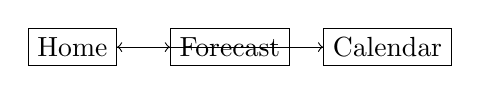
\begin{tikzpicture}[node distance=2cm, auto]
    \node (home) [draw, rectangle] {Home};
    \node (forecast) [draw, rectangle, right of=home] {Forecast};
    \node (calendar) [draw, rectangle, right of=forecast] {Calendar};
    \draw[->] (home) -- (forecast);
    \draw[->] (forecast) -- (calendar);
    \draw[->] (calendar) -- (home);
  \end{tikzpicture}
  \caption{Primary navigation: Home $\to$ Forecast $\to$ Calendar.}
\end{figure}

\section{Design Decisions and Rationale}

\subsection{Layout}
CSS Grid for desktop (three columns), Flexbox for mobile stack.

\subsection{Color \& Theme}
Neutral base palette, blue accent for weather, orange for actions; dark mode inverts background/text. Contrast $\geq$\,4.5:1 at all breakpoints.

\subsection{Typography}
Sans-serif (e.g.\ \texttt{Open Sans}) at 16\,px base, headings at 20--24\,px.

\subsection{Interactions}
\begin{itemize}[nosep]
  \item Loading spinner during data fetch.
  \item Date click opens side panel with details.
  \item Toggles persist via localStorage.
\end{itemize}

\subsection{Accessibility}
\begin{itemize}[nosep]
  \item ARIA labels on interactive elements.
  \item Keyboard navigation \& visible focus indicators.
  \item Zoom support up to 200\% without breaking layout.
\end{itemize}

\section{Responsiveness \& Accessibility}

\textbf{Breakpoints:}
\begin{itemize}[nosep]
  \item Mobile: <\,600\,px
  \item Tablet: 600--1023\,px
  \item Desktop: $\geq$\,1024\,px
\end{itemize}
Adaptive layout: stacked $\to$ two-column $\to$ three-pane. Maintain contrast ratios $\geq$\,4.5:1; announce data loads for screen readers.

\section{Acknowledgement of AI Tools}
Drafted with GPT-4o for structure; all wireframes and decisions reviewed and refined by the team.

\end{document}
